\documentclass[a4paper]{article}
\usepackage{color}              %Farben, f.r \definecolor{}
\usepackage{amssymb}            %Mathematische Symbole
\usepackage{amsthm}             %Besseres \newtheorem
\usepackage{amsmath}           %Mathematische Umgebungen
\usepackage{mathtools}          %\xRightarrow, etc
\usepackage{mathrsfs}           %enthaelt \mathscr
\usepackage{graphicx}
\usepackage{enumerate}          % in-place numerations def.
\usepackage{fullpage}
\usepackage{hyperref}

\usepackage{array}
%\usepackage{multicol}
%\usepackage[notref,notcite]{showkeys}
%\usepackage{algorithm,algorithmic}
\usepackage{color}

\usepackage{graphicx}
\usepackage{xypic}
\entrymodifiers={+!!<0pt,\fontdimen22\textfont2>}
\usepackage[all]{xy}

\usepackage{float}
\usepackage{tikz}
\usepackage{tikz-cd}
\usepackage{tikz,fullpage}
\usetikzlibrary{arrows,%
                petri,%
                topaths}%
\usepackage{tkz-berge}
\usepackage[position=top]{subfig}
\usetikzlibrary{shapes.geometric}
\usetikzlibrary{decorations.markings}

\newtheoremstyle{myremark} % name
    {7pt}                    % Space above
    {7pt}                    % Space below
    {}  	                 % Body font
    {}                           % Indent amount
    {\bf}       	         % Theorem head font
    {.}                          % Punctuation after theorem head
    {.5em}                       % Space after theorem head
    {}  % Theorem head spec (can be left empty, meaning �normal�)

\theoremstyle{plain}
\newtheorem{lemma}{Lemma}
\newtheorem{theorem}[lemma]{Theorem}
\newtheorem{fact}[lemma]{Fact}
\newtheorem{definition}[lemma]{Definition}
\newtheorem{corollary}[lemma]{Corollary}
\newtheorem{proposition}[lemma]{Proposition}
\newtheorem{conjecture}[lemma]{Conjecture}
\newtheorem{observation}[lemma]{Observation}
\newtheorem{problem}[lemma]{Problem}
\newtheorem{notation}[lemma]{Notation}
\newtheorem*{claim}{Claim}

\theoremstyle{myremark}
\newtheorem{remark}[lemma]{Remark}
\newtheorem{example}[lemma]{Example}
\newtheorem{exercise}[lemma]{Exercise}
\newtheorem{algorithm}[lemma]{Algorithm}
\newtheorem{application}[lemma]{Application}
\newtheorem*{goal}{Goal}

%%%%%% EDIT HERE: %%%%%%%%%%%
\newcommand{\LECTURENUMBER}{0}
\newcommand{\LECTURETITLE}{Short title}
\newcommand{\LECTURESCRIBE}{Your name}

%% Dokument Beginn %%%%%%%%%%%%%%%%%%%%%%%%%%%%%%%%%%%%%%%%%%%%%%%%%%%%%%%%
\begin{document}
\thispagestyle{empty}

\begin{center}
	{\Large\bf Graph coloring}\\
	{\bf Lecture notes, vol. 4 \\ Accuracy of lower bounds, probabilistic method and $\chi$ of some constructions}\\
\end{center}
Lecturer: Michal Adamaszek \hfill Scribe: Mathis Isaksen
\begin{center}
\line(1,0){450}
\end{center}

%%%%%%% EDIT ALSO BELOW: %%%%%%%%%%%%%%%%
\section*{Accuracy of lower bounds}
We know that $\chi(G)\geq\omega(G)$ \\
If $G=C_{2n+1}, \quad n\geq 2$ then $\omega(G)=2,\quad \chi(G)=3$ \\
Q: Is there a graph with $\omega(G)=2$ and $\chi(G)=4$? \\
A: Yes the smallest such is the Gr{\"o}tszch graph on 11 vertices $G_{11}$ \\
\href{https://en.wikipedia.org/wiki/Gr�tzsch_graph}{https://en.wikipedia.org/wiki/Gr{\"o}tzsch{\_}graph} \\
\\
It is not possible to bound $\chi(G)$ in terms of $\omega(G)$.
\begin{theorem} 
For any $k\geq2$ there is a triangle-free graph with $\chi(G)=k$
\end{theorem}
\begin{definition}
Suppose $G$ is a graph with $V(G)=\{v_1,..,v_n\}$. The \emph{Mycielski construction} $M(G)$ is a new graph with $V(M(G))=\{v_1 ,..,v_n\}\cup\{u_1,..,u_n\}\cup\{w\}, \quad E(M(G))=\{wu_i,\, i=1,..,n\} \cup \{v_i v_j,\ u_iv_j\ : v_iv_j \in E(G)\}$.

\begin{figure}[H]
\begin{center}
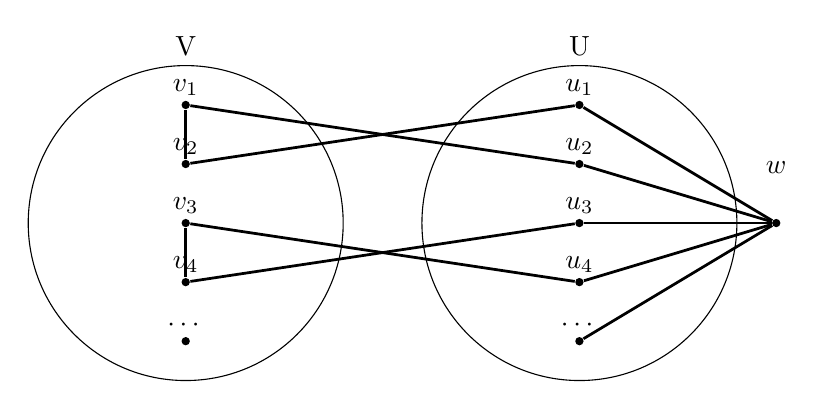
\begin{tikzpicture} 
\draw (-2.5,0) circle (2) (-2.5,2)  node [text=black,above] {V}
      (2.5,0) circle (2) (2.5,2)  node [text=black,above] {U}
			node[fill,circle,inner sep=0pt,minimum size=3pt] (nw) at (5,0) {} 
(5,0.5) node [text=black,above] {$w$};

\draw  
node[fill,circle,inner sep=0pt,minimum size=3pt] (n1) at (-2.5,1.5) {} 
(-2.5,1.5) node [text=black,above] {$v_1$}
	node[fill,circle,inner sep=0pt,minimum size=3pt] (n2) at (-2.5,0.75) {} 
(-2.5,0.75) node [text=black,above] {$v_2$}
	node[fill,circle,inner sep=0pt,minimum size=3pt] (n3) at (-2.5,0) {} 
(-2.5,0) node [text=black,above] {$v_3$}
	node[fill,circle,inner sep=0pt,minimum size=3pt] (n4) at (-2.5,-0.75) {} 
(-2.5,-0.75) node [text=black,above] {$v_4$}
	node[fill,circle,inner sep=0pt,minimum size=3pt] (n5) at (-2.5,-1.5) {} 
(-2.5,-1.5) node [text=black,above] {$\cdots$}

	node[fill,circle,inner sep=0pt,minimum size=3pt] (n6) at (2.5,1.5) {} 
(2.5,1.5) node [text=black,above] {$u_1$}
	node[fill,circle,inner sep=0pt,minimum size=3pt] (n7) at (2.5,0.75) {} 
(2.5,0.75) node [text=black,above] {$u_2$}
	node[fill,circle,inner sep=0pt,minimum size=3pt] (n8) at (2.5,0) {} 
(2.5,0) node [text=black,above] {$u_3$}
	node[fill,circle,inner sep=0pt,minimum size=3pt] (n9) at (2.5,-0.75) {} 
(2.5,-0.75) node [text=black,above] {$u_4$}
	node[fill,circle,inner sep=0pt,minimum size=3pt] (n10) at (2.5,-1.5) {} 
(2.5,-1.5) node [text=black,above] {$\cdots$};

\draw [line width = 1 pt, black, -] (n6) edge node {} (nw)
 	[line width = 1 pt, black, -] (n7) edge node {} (nw)
 	 [line width = 1 pt, black, -] (n8) edge node {} (nw)
  	 [line width = 1 pt, black, -] (n9) edge node {} (nw)
 	 [line width = 1 pt, black, -] (n10) edge node {} (nw)
	[line width = 1 pt, black, -] (n1) edge node {} (n2)
	[line width = 1 pt, black, -] (n6) edge node {} (n2)
	[line width = 1 pt, black, -] (n7) edge node {} (n1)
	[line width = 1 pt, black, -] (n3) edge node {} (n4)
	[line width = 1 pt, black, -] (n3) edge node {} (n9)
	[line width = 1 pt, black, -] (n4) edge node {} (n8)
	;
\end{tikzpicture}
\end{center}
\end{figure}
\end{definition}

As an example have that $M(K_2)=C_5$ and $M(C_5)=G_{11}$.

\begin{theorem} (restated) If $G$ is triangle-free and $\chi(G)=k$ then $M(G)$ is triangle free and $\chi(M(G))=k+1$.
\end {theorem}
\begin{proof}
\begin{enumerate}
	\item $M(G)$ is still triangle free \\
	The only possibility is a triangle with $1$ vertex from $U$ and 2 vertices from $V$. However, by the definition of $M(G)$ we then have that $v_iv_jv_k$ is a triangle, contradicting that $G$ was triangle-free.
	\item $M(G)$ is $k+1$ colorable \\
	We can color $G$ with $k$ colors (The set $V$ in the picture). We use another color $(k+1)$ for all vertices in $U$, and the last node $w$ is colored with some color different from $(k+1)$ 
	\item $M(G)$ is not $k$-colorable. \\
	Suppose otherwise, $c:V(M(G)) \rightarrow \{1,..,k\}$. Suppose wlog that $w$ has color $k$, then $U$ is colored with $k-1$ colors. (Our goal is to show that we can color $G$ with $k-1$ colors) \\
	Let $A= \{v_i \in V, \, c(v_i)=k\}$. \\
	Recolor $A$ by changing the color of each $v_i$ to $c(u_i)$ \\
	$$
	c'(v_i)=\left\{ \begin{array}{rl}
c(v_i) &\mbox{ if $c(v_i)\neq k$} \\
c(u_i) &\mbox{ if $c(v_i)=k$}
\end{array} \right.
$$
$C'$ uses only colors $ \{1,..,k-1\} $. Let's check that $c'$ is a coloring of $G$. Suppose $c'(v_i)=c'(v_j)$ 
\begin{enumerate}
	\item If both of these $v_i,v_j \notin A$ then $v_iv_j \notin E(G)$  
	\item If $v_i \in A,\, v_j \notin A$. Suppose $v_iv_j \in E(G)$, so that $u_iv_j \in E(M(G))$
	\begin{figure}[H]
\begin{center}
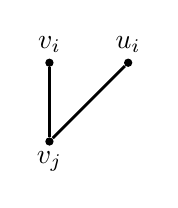
\begin{tikzpicture} 

		

\draw  
node[fill,circle,inner sep=0pt,minimum size=3pt] (n1) at (0,0.5) {} 
(0,0.5) node [text=black,above] {$v_i$}
	node[fill,circle,inner sep=0pt,minimum size=3pt] (n2) at (0,-0.5) {} 
(0,-0.5) node [text=black,below] {$v_j$}
	node[fill,circle,inner sep=0pt,minimum size=3pt] (n3) at (1,0.5) {} 
(1,0.5) node [text=black,above] {$u_i$};


\draw [line width = 1 pt, black, -] (n1) edge node {} (n2)
 	[line width = 1 pt, black, -] (n2) edge node {} (n3)
 	
	;
\end{tikzpicture}
\end{center}
\end{figure}
Then $c(u_i)=c'(v_i)=c'(v_j)=c(v_j)$ Contradicting that $c$ is a coloring of $M(G)$
	\item If $v_i,v_j \in A$. Then $c(v_i)=c(v_j)=k \Rightarrow v_iv_j \notin E(G)$
\end{enumerate}
\end{enumerate}
\end{proof}

Recap: We can have triangle-free graphs with arbitrarily high $\chi$. But is $M(G)$ just a special construction that achieves this? Not really. We will see that in the following:
\section*{Probabilistic method} 
Goal: Prove that objects with an interesting property $P$ exists by showing that a random object has $P$ with non-zero probability. For example: $P=$"triangle-free and $\chi(G)\geq k$"

\begin{definition} (construction). Fix $V=\{1,..,n\}, \, 0\leq p\leq 1$. Construct a graph on $V$ by taking each edge $ij$, $0 \leq i <j \leq n$ with probability $p$, independently for each each pair. \\
$G(n,p)$ is the probability space of all graphs obtained in this way.

\end{definition}

A graph $G \in G(n,p)$ has probability
$$
\mathbb{P}(G)=p^{|E(G)|}(1-p)^{\binom{n}{2}-|E(G)|}.
$$
The expected number of edges/triangles in a random graph from $G(n,p)$ is
$$
\mathbb{E}[\# \text{edges}]=\binom{n}{2}\mathbb{P}[ij \text{ is an edge}]=p\binom{n}{2}
$$
$$
\mathbb{E}[\# \text{of triangles in } G(n,p)]=\binom{n}{3}\mathbb{P}[ijk \text{ is a triangle}]=\binom{n}{3}p^3
$$
Sage can generate random graphs from $G(n,p)$ (\texttt{graphs.randomGNP(n, p)}). 
For the next part we need a few prerequisites:
\begin{enumerate}
	\item $1-x \leq e^{-x}$,
	\item $\binom{n}{k} \leq n^k$,
	\item Markov's inequality: if $X$ is a non-negative random variable, $t>0$, then $\mathbb{P}[X>t]\leq \frac{1}{t}\mathbb{E}[X]$.
\end{enumerate}
\begin{theorem} For every $k\geq 2$  there is a triangle-free graph with $\chi(G)\geq k$.
\end{theorem}
Remark: Not only "there is" but "there are many".
\begin{proof}
Take $G \in G(n,p)$ where $p=\frac{1}{n^{5/6}}$. Let $X=\#$ of triangles in $G$. \\
$\mathbb{E}[X]=\binom{n}{3}p^3 \leq n^{1/2}$. By Markov's inequality $\mathbb{P}[X>10n^{1/2}]\leq \frac{1}{10}$, which means that a typical $G$ has very few triangles. \\
To show that $\chi(G)$ is "large" we will prove that $\alpha(G)$ is "small". Let $a=\frac{3}{p}\ln{n}$ 
$$
\mathbb{P}[\alpha(G)\geq a] \leq \binom{n}{a}\mathbb{P}[\text{exists independent set of size }a] = \binom{n}{a}(1-p)^{\binom{a}{2}} \leq n^ae^{-p\binom{a}{2}} \rightarrow 0,\quad n\rightarrow \infty
$$
where the last limit can be computed by plugging in the formulae for $p$ and $a$ in terms of $n$.

For sufficiently large $n$ we have $\mathbb{P}[\alpha(G)\geq a]<\frac{1}{10}$. Then $$\mathbb{P}[X<10\sqrt{n} \text{ and } \alpha(G)<a] \geq \frac{8}{10}.$$

We showed, with probability $\geq \frac{8}{10}$, a random graph from $G(n,p), \, p=\frac{1}{n^{5/6}}$, has $<10\sqrt{n}$ triangles, and $\alpha(G)<a<3n^{5/6}\ln{n}$ \\
Completing the proof: \\
Take such a random $G$. Remove at most $10\sqrt{n}$ vertices so we get a triangle free graph $G'$ \\
$|V(G')| \geq \frac{n}{2}$ (for large $n$) and 
$$
\chi(G')\geq \frac{|V(G')|}{\alpha(G')} \geq \frac{n/2}{3n^{5/6}\ln{n}}=\frac{1}{6}\frac{n^{1/6}}{\ln{n}}\rightarrow \infty, \quad n\rightarrow \infty
$$
So $\chi(G')$ can be arbitrarily large
\end{proof}

\section*{$\chi$ of some constructions on graphs}
\begin{enumerate}
	\item Disjoint union $G \sqcup H$. $\chi(G \sqcup H)=\max(\chi(G),\chi(H))$. As $G\subseteq G \sqcup H \supseteq H$, we need at least enough colors to color $H,G$ individually.
	\item Wedge $G \vee H$ Graphs joined at a single vertex.

\begin{figure}[H]
\begin{center}
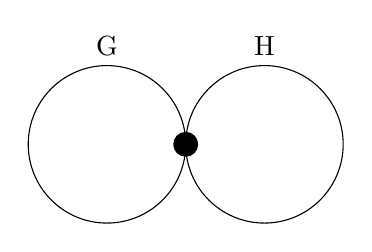
\begin{tikzpicture}	
\draw (-1.0,0) circle (1) (-1.0,1)  node [text=black,above] {G}
      (1.0,0) circle (1) (1.0,1)  node [text=black,above] {H}
			node[fill,circle,inner sep=0pt,minimum size=9pt] (nw) at (0,0) {};

\end{tikzpicture}
\end{center}
\end{figure}

$\chi(G\vee H)=\max(\chi(G),\chi(H)$. After coloring $G$ color $H$, perhaps permuting the colors so that they agree on the common vertex..	
	
\item The sum (join) $G+H$. It is the disjoint union together with all edges between $V(G)$ and $V(H)$ \\
$\chi(G+H)=\chi(G)+\chi(H)$. As the colors of $G$ must be different from the colors of $H$.
\item The cartesian product $G \square H$ \\
$V(G \square H) = V(G) \times V(H)$ \\
$\{(u,v),(u',v')\} \text{ is an edge iff } (u=u' \text{ and } vv' \in E(H)) \text{ or } (uu' \in E(G) \text{ and } v=v')$. 

\begin{lemma} $\chi(G \square H)=\max(\chi(G),\chi(H))$
\end{lemma}
\begin{proof}
$G\subseteq G \square H \supseteq H$ so $\chi(G \square H) \geq \max(\chi(G),\chi(H))$. Suppose $G$ and $H$ both have coloring with color set $\{0,..,k-1\}$ ($k=\max(\chi(G), \chi(H))$). Le these colorings be 
$$
f: V(G) \rightarrow \{ 0,..,k-1\},
$$
$$
f': V(H) \rightarrow \{ 0,..,k-1 \}.
$$
Define $F(u,v)=f(u)+f'(v) \mod k$. We will check that $F$ is a coloring. Let $(u,v)(u',v') \in E(G \square H)$. Wlog let $u=u'$ and $vv' \in E(H)$, then:
\begin{align*}
	F(u,v) &=f(u)+f'(v) \mod k \\
	F(u',v') &=f(u')+f'(v') \mod k \\
	         &= f(u)+f'(v') \mod k \\
					&\neq f(u)+f'(v) \mod k  \quad \text{because } vv' \in E(H) \\
					&=F(u,v).
\end{align*}
\end{proof}
As an exercise, show that $\chi(G)\geq h$ iff $\alpha(G \square K_k) \geq |V(G)|$.
\end{enumerate}

\end{document}


